\subsubsection{Justage und Einstellung der Startparameter}
\noindent Zu Beginn des Versuchs wird die Temperatur am Ort der Probe mittels
des Thermometers gemessen. Anschließend wird eine Referenzprobe in die Spule im
Permanentmagneten eingesetzt und die Justage vorgenommen. Die Referenzprobe
besteht aus Wasser versetzt mit Kupfersulfat (CuSO$_4$), welches eine kürzere
Relaxationszeit als eine Probe aus reinem Wasser besitzt. Für die Startparameter
der Messung sind dabei die Frequenz $f = \SI{21.7}{\mega\hertz}$, die Pulslänge des $\SI{90}{\degree}$-Pulses $t_A =
\SI{2}{\micro\second}$, die Anzahl der $\SI{180}{\degree}$-Pulse $N_B = 0$, sowie die Periodendauer
$P = \SI{0.5}{\second}$ und die Shims-Parameter $x = -0.1, y = -5.0, z = 3.7$
und $z^2 = -2.4$ am Steuergerät einzustellen. Eine Darstellung der Pulse und
Pulsabstände ist in Abbildung \ref{fig:pulse} gegeben. \\
\FloatBarrier
\begin{figure}
  \centering
  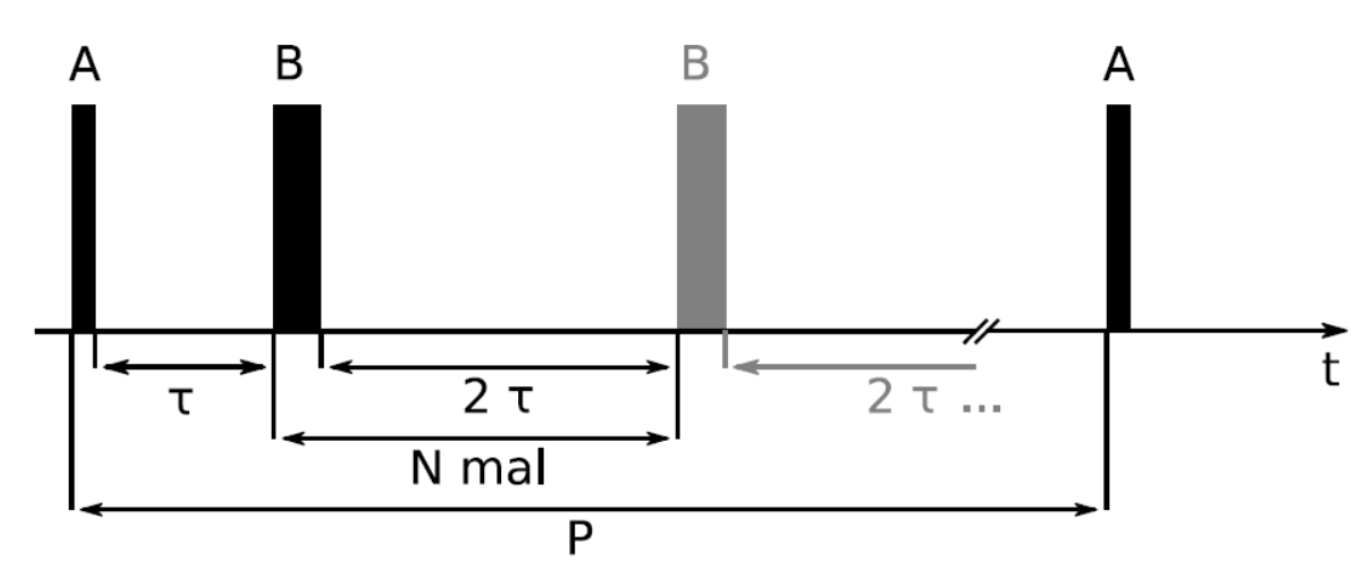
\includegraphics[scale=0.3]{resources/pulse.png}
  \caption{Schematische Darstellung des Pulsprogramms nach \cite{sample}.}
  \label{fig:pulse}
\end{figure}
\FloatBarrier
\noindent Bei der Justage der Frequenz ist
zu beachten, dass die Detektion von Real- und Imaginärteil relativ zur
Lamorfrequenz geschieht und dass die Frequenz dann korrekt justiert ist, wenn
keine Schwingungen des Signals mehr messbar sind. Um einen deutlichen
Signaleingang zu erhalten, ist die Phase so zu wählen, dass der Imaginärteil
verschwindet und das Signal im Realteil angetragen wird. Durch die
Shim-Parameter wird die Feldhomogenität der Spule maximiert, die Pulslänge
für einen $\alpha = \SI{90}{\degree}$ Puls wird ein Wert gesucht, für welchen
der freie Induktionsfall maximal wird. Als Startparameter dient eine Pulslänge
von $\SI{2}{\micro\second}$ zur Orientierung, für einen $\alpha = \SI{180}{\degree}$ Puls
ist die Pulslänge etwa doppelt so lang. \\
\subsubsection{Messung der Spin-Gitter-Relaxationszeit}
Zur Messung der Spin-Gitter-Relaxationszeit $T_1$ werden die $\SI{90}{\degree}$-Pulse,
welche einen freien Induktionsfall anregen auf eine Länge von $t_A =
\SI{2}{\micro\second}$ eingestellt. Die für eine Spiegelung der Kernspin-Momente
zuständigen $\SI{180}{\degree}$-Pulse werden auf eine Länge $t_B =
\SI{4}{\micro\second}$ eingestellt und einmalig ausgeführt. Für die Periode ist eine
Dauer von $P = \SI{10}{\second}$ zu wählen, eine Nachjustage ist erforderlich,
sobald der Abstand $\tau$ zwischen den Pulsen mehr als eine Sekunde beträgt. In
diesem Fall ist eine Periodendauer $P + \tau$ zu wählen. Variiert werden soll in
der Messung der Pulsabstand $\tau$, während die Spannung des FID nach dem
$\SI{90}{\degree}$-Puls gemessen wird. \\
\noindent Die im freien Induktionsfall entstehende Schwingung des
Induktionsstromes klingt mit der Zeit ab und wird gemessen. Bei der Messung ist
darauf zu achten, dass $t$ so gewählt wird, dass für den kürzesten Abstand
noch keine Relaxation stattgefunden hat, die Magnetisierung der Probe für den
längsten Abstand allerdings vollständig relaxiert ist. Des Weiteren ist die
Messung bis weit über den Nulldurchgang hinaus durchzuführen. \\
\subsubsection{Messung der Spin-Spin-Relaxationszeit}
\noindent Um die Spin-Spin-Relaxationszeit zu bestimmen, werden die Längen der
$\SI{90}{\degree}$- und $\SI{180}{\degree}$-Pulse eingestellt und die Anzahl der
Wiederholungen der $\SI{180}{\degree}$-Pulse auf
$N_B = 100$ gesetzt. Die Periodendauer soll dazu mindestens $P = 3 \cdot T_1$
betragen. Um eine Phasenverschiebung von $\Delta \phi = \SI{90}{\degree}$
zwischen den $\SI{90}{\degree}$-Pulse und $\SI{180}{\degree}$-Pulsezu erreichen,
wird der Schalter \enquote{MG} auf
\enquote{on} gestellt. Der Abstand der Pulse untereinander ist so zu wählen,
dassdas Maximum des letzten Echosignals etwa $\frac{1}{3}$ des ersten Maximums
beträgt. Zur Auswertung wird ein Bild des Ozsilloskops gespeichert. Anschließend
wird diese Messung für die Schalterstellung \enquote{MG off} wiederholt. \\
\noindent Zum Abschluss wird das Phänomen der Diffusion untersucht. Dazu wird
mithilfe der Shim-Einstellung durch Umpolung  und Maximierung des z-Gradienten
das Gradientenfeld erhöht, die $\SI{90}{\degree}$- und $\SI{180}{\degree}$-Pulse
bleiben wie vorab eingestellt. Der $\SI{180}{\degree}$-Puls wird einmalig ausgeführt und erfährt
keine Wiederholung. Die Periodendauer bleibt auf dem vorher eingestellten Wert.
Über mehrere Größenordnungen hinweg wird anschließend der Pulsabstand $\tau$
ausgehend von $\tau = \SI{100}{\micro\second}$ variiert. Die gemessenen Echosignale
werden als .csv-Dateien vom Oszilloskop auf ein Speichermedium übertragen.
\subsubsection{Hahn-Echo-Verfahren}
\noindent Um die Spin-Spin-Relaxationszeit $T_2$ zu bestimmen, werden
aufeinander verschiedene Verfahren angewendet. Beim Hahn-Echo-Verfahren werden
Feldinhomogenitäten durch Ausnutzung der FID kompensiert. Ein $\SI{90}{\degree}$-Puls regt den
FID an, ein $\SI{180}{\degree}$-Puls spiegelt die Auslenkung des Signals an der y-Achse.
Divergierende Spins konvergieren dadurch wieder und es entsteht ein Echo. Die
Messung der Amplituden erfolgt dabei in einem Abstand von $2 \cdot \tau$. Eine
Erweiterung dieses Messverfahrens ist das Carr-Purcell-Messverfahren. In diesem
wird anstelle von einem Signalecho im Abstand $2 \cdot \tau$ eine Vielzahl
dieser Echosignale betrachtet. Problematisch dabei ist allerdings, dass eine
nur gering von der theoretischen Pulslänge abweichende tatsächliche
Pulslänge nicht gänzlich zur Spiegelung des Signals an der y-Achse führt und
so eine mit jedem Schritt ansteigende Messunsicherheit verursacht. Stehen die
$\SI{180}{\degree}$-Pulse allerdings mit einem Versatz von $\Delta \phi = \SI{90}{\degree}$ zu den
$\SI{90}{\degree}$-Pulsen, so löschen sich die entstehenden Unsicherheiten bei jeder Spiegelung
selbst aus, für Gesamtpulslängen ganzzahliger Vielfacher von $4 \cdot \tau$
werden korrigierte Werte gemessen. Dieses Verfahren wird auch
Meiboom-Gill-Verfahren genannt. \\
